% Options for packages loaded elsewhere
\PassOptionsToPackage{unicode}{hyperref}
\PassOptionsToPackage{hyphens}{url}
\documentclass[
]{article}
\usepackage{xcolor}
\usepackage{amsmath,amssymb}
\setcounter{secnumdepth}{-\maxdimen} % remove section numbering
\usepackage{iftex}
\ifPDFTeX
  \usepackage[T1]{fontenc}
  \usepackage[utf8]{inputenc}
  \usepackage{textcomp} % provide euro and other symbols
\else % if luatex or xetex
  \usepackage{unicode-math} % this also loads fontspec
  \defaultfontfeatures{Scale=MatchLowercase}
  \defaultfontfeatures[\rmfamily]{Ligatures=TeX,Scale=1}
\fi
\usepackage{lmodern}
\ifPDFTeX\else
  % xetex/luatex font selection
\fi
% Use upquote if available, for straight quotes in verbatim environments
\IfFileExists{upquote.sty}{\usepackage{upquote}}{}
\IfFileExists{microtype.sty}{% use microtype if available
  \usepackage[]{microtype}
  \UseMicrotypeSet[protrusion]{basicmath} % disable protrusion for tt fonts
}{}
\makeatletter
\@ifundefined{KOMAClassName}{% if non-KOMA class
  \IfFileExists{parskip.sty}{%
    \usepackage{parskip}
  }{% else
    \setlength{\parindent}{0pt}
    \setlength{\parskip}{6pt plus 2pt minus 1pt}}
}{% if KOMA class
  \KOMAoptions{parskip=half}}
\makeatother
\usepackage{longtable,booktabs,array}
\newcounter{none} % for unnumbered tables
\usepackage{calc} % for calculating minipage widths
% Correct order of tables after \paragraph or \subparagraph
\usepackage{etoolbox}
\makeatletter
\patchcmd\longtable{\par}{\if@noskipsec\mbox{}\fi\par}{}{}
\makeatother
% Allow footnotes in longtable head/foot
\IfFileExists{footnotehyper.sty}{\usepackage{footnotehyper}}{\usepackage{footnote}}
\makesavenoteenv{longtable}
\usepackage{graphicx}
\makeatletter
\newsavebox\pandoc@box
\newcommand*\pandocbounded[1]{% scales image to fit in text height/width
  \sbox\pandoc@box{#1}%
  \Gscale@div\@tempa{\textheight}{\dimexpr\ht\pandoc@box+\dp\pandoc@box\relax}%
  \Gscale@div\@tempb{\linewidth}{\wd\pandoc@box}%
  \ifdim\@tempb\p@<\@tempa\p@\let\@tempa\@tempb\fi% select the smaller of both
  \ifdim\@tempa\p@<\p@\scalebox{\@tempa}{\usebox\pandoc@box}%
  \else\usebox{\pandoc@box}%
  \fi%
}
% Set default figure placement to htbp
\def\fps@figure{htbp}
\makeatother
\setlength{\emergencystretch}{3em} % prevent overfull lines
\providecommand{\tightlist}{%
  \setlength{\itemsep}{0pt}\setlength{\parskip}{0pt}}
\usepackage{bookmark}
\IfFileExists{xurl.sty}{\usepackage{xurl}}{} % add URL line breaks if available
\urlstyle{same}
\hypersetup{
  pdftitle={Posterior-Based Decision Stability in Urban Flood Risk Prioritisation},
  hidelinks,
  pdfcreator={LaTeX via pandoc}}

\title{Posterior-Based Decision Stability in Urban Flood Risk
Prioritisation}
\author{Mikel Martinez Mugica\\
Independent Researcher\\
https://habnetic.org}
\date{April 2026}

\begin{document}
\maketitle

\subsection{Abstract}\label{abstract}

Urban risk assessments often produce ranked lists of assets or locations
to guide infrastructure investment and resilience planning. These
rankings are typically derived from deterministic risk scores or
expected impact estimates. While uncertainty may be quantified within
individual model components, it is rarely propagated through the full
exposure--hazard--impact chain to the prioritisation decisions
themselves.

This paper introduces a reproducible Bayesian baseline for propagating
uncertainty from exposure and hazard proxies to decision-relevant
prioritisation metrics in urban pluvial risk assessment. This allows
prioritisation decisions themselves to be analysed as random variables
derived from the posterior, rather than fixed rankings derived from
uncertain inputs.

Using Rotterdam as a case study (\textasciitilde221,324 buildings), we
construct an exposure--hazard--outcome pipeline and perform Bayesian
inference to estimate posterior distributions of asset-level impact
probabilities. Prioritisation decisions are then derived from posterior
draws rather than point estimates.

We quantify decision stability using posterior-derived metrics including
top-k membership probability and borderline share. Results indicate that
most assets exhibit stable prioritisation outcomes under the current
modelling assumptions, while a small fraction occupy a narrow decision
boundary where ranking uncertainty is concentrated. This structure is
further shown to be robust under controlled perturbations of the hazard
proxy, suggesting that the observed decision boundary is not driven by
deterministic hazard specification.

This work provides a minimal probabilistic baseline for analysing
decision stability in urban risk prioritisation and establishes a
foundation for later extensions incorporating hazard uncertainty and
cross-city transfer.

\begin{center}\rule{0.5\linewidth}{0.5pt}\end{center}

\section{1. Introduction}\label{introduction}

Urban resilience planning frequently relies on ranked lists of assets
requiring intervention, such as buildings, infrastructure segments, or
neighbourhoods. These rankings typically emerge from deterministic risk
scores or expected damage estimates. In practice, these rankings
directly determine which assets receive intervention under limited
budgets, making their stability a critical but often unexamined
property.

However, risk estimation involves substantial uncertainty arising from:

\begin{itemize}
\tightlist
\item
  hazard variability
\item
  exposure measurement error
\item
  model specification
\item
  limited observational data
\end{itemize}

Although uncertainty may be analysed within individual modelling
components, it is rarely propagated through the full modelling chain to
the final prioritisation decisions.

As a result, the stability of ranked intervention lists remains largely
unexplored.

This paper proposes treating \textbf{prioritisation stability itself as
the primary inferential object}. While uncertainty propagation has been
widely studied within individual components of flood risk models,
particularly in Bayesian flood damage modelling and hydrological
ensemble simulations (Sairam et al., 2019; Mohor et al., 2021; McMillan
\& Brasington, 2008), the stability of the resulting prioritisation
decisions has received comparatively little attention.

Instead of asking only:

\begin{quote}
Which assets appear most at risk?
\end{quote}

we ask:

\begin{quote}
How stable are prioritisation decisions when uncertainty is propagated
through the modelling pipeline?
\end{quote}

To explore this question, we construct a reproducible Bayesian baseline
for urban pluvial risk assessment and derive prioritisation metrics
directly from posterior distributions.

The contribution of this paper is therefore methodological: rather than
improving hazard or damage estimation alone, the framework evaluates how
uncertainty propagates into the stability of prioritisation decisions
themselves.

\subsubsection{Contributions}\label{contributions}

This paper makes three main contributions:

\begin{itemize}
\tightlist
\item
  A reproducible \textbf{exposure--hazard--outcome modelling pipeline}
\item
  A \textbf{Bayesian inference baseline} for asset-level impact
  probability
\item
  A set of \textbf{posterior-derived prioritisation metrics} for
  quantifying decision stability
\end{itemize}

These contributions are demonstrated through a citywide decision
stability analysis for Rotterdam (\textasciitilde221k assets). The
framework is further designed for later transfer to Hamburg and
Donostia--San Sebastián.

\begin{center}\rule{0.5\linewidth}{0.5pt}\end{center}

\section{2. Conceptual Framework}\label{conceptual-framework}

Urban flood risk assessments typically follow a conceptual structure
linking:

Exposure → Hazard → Impact (Outcome)

where exposure describes asset characteristics, hazard represents
environmental forcing, and impact represents realised damage or
disruption.

Probabilistic approaches to flood risk modelling have previously been
applied to individual components of this chain, including Bayesian
damage estimation (Sairam et al., 2019; Mohor et al., 2021) and
probabilistic flood susceptibility models using Bayesian networks (Wu et
al., 2019, 2020).

In probabilistic terms this can be expressed as a generative model:

Data → Exposure → Hazard → Outcome\\
→ Posterior inference\\
→ Decision metrics

Posterior inference produces distributions over model parameters and
asset-level risk probabilities. Rather than collapsing these
distributions to point estimates, we derive decision quantities directly
from the posterior.

This allows prioritisation decisions to be analysed probabilistically.

\subsubsection{Graphical model}\label{graphical-model}

\begin{figure}
\centering
\pandocbounded{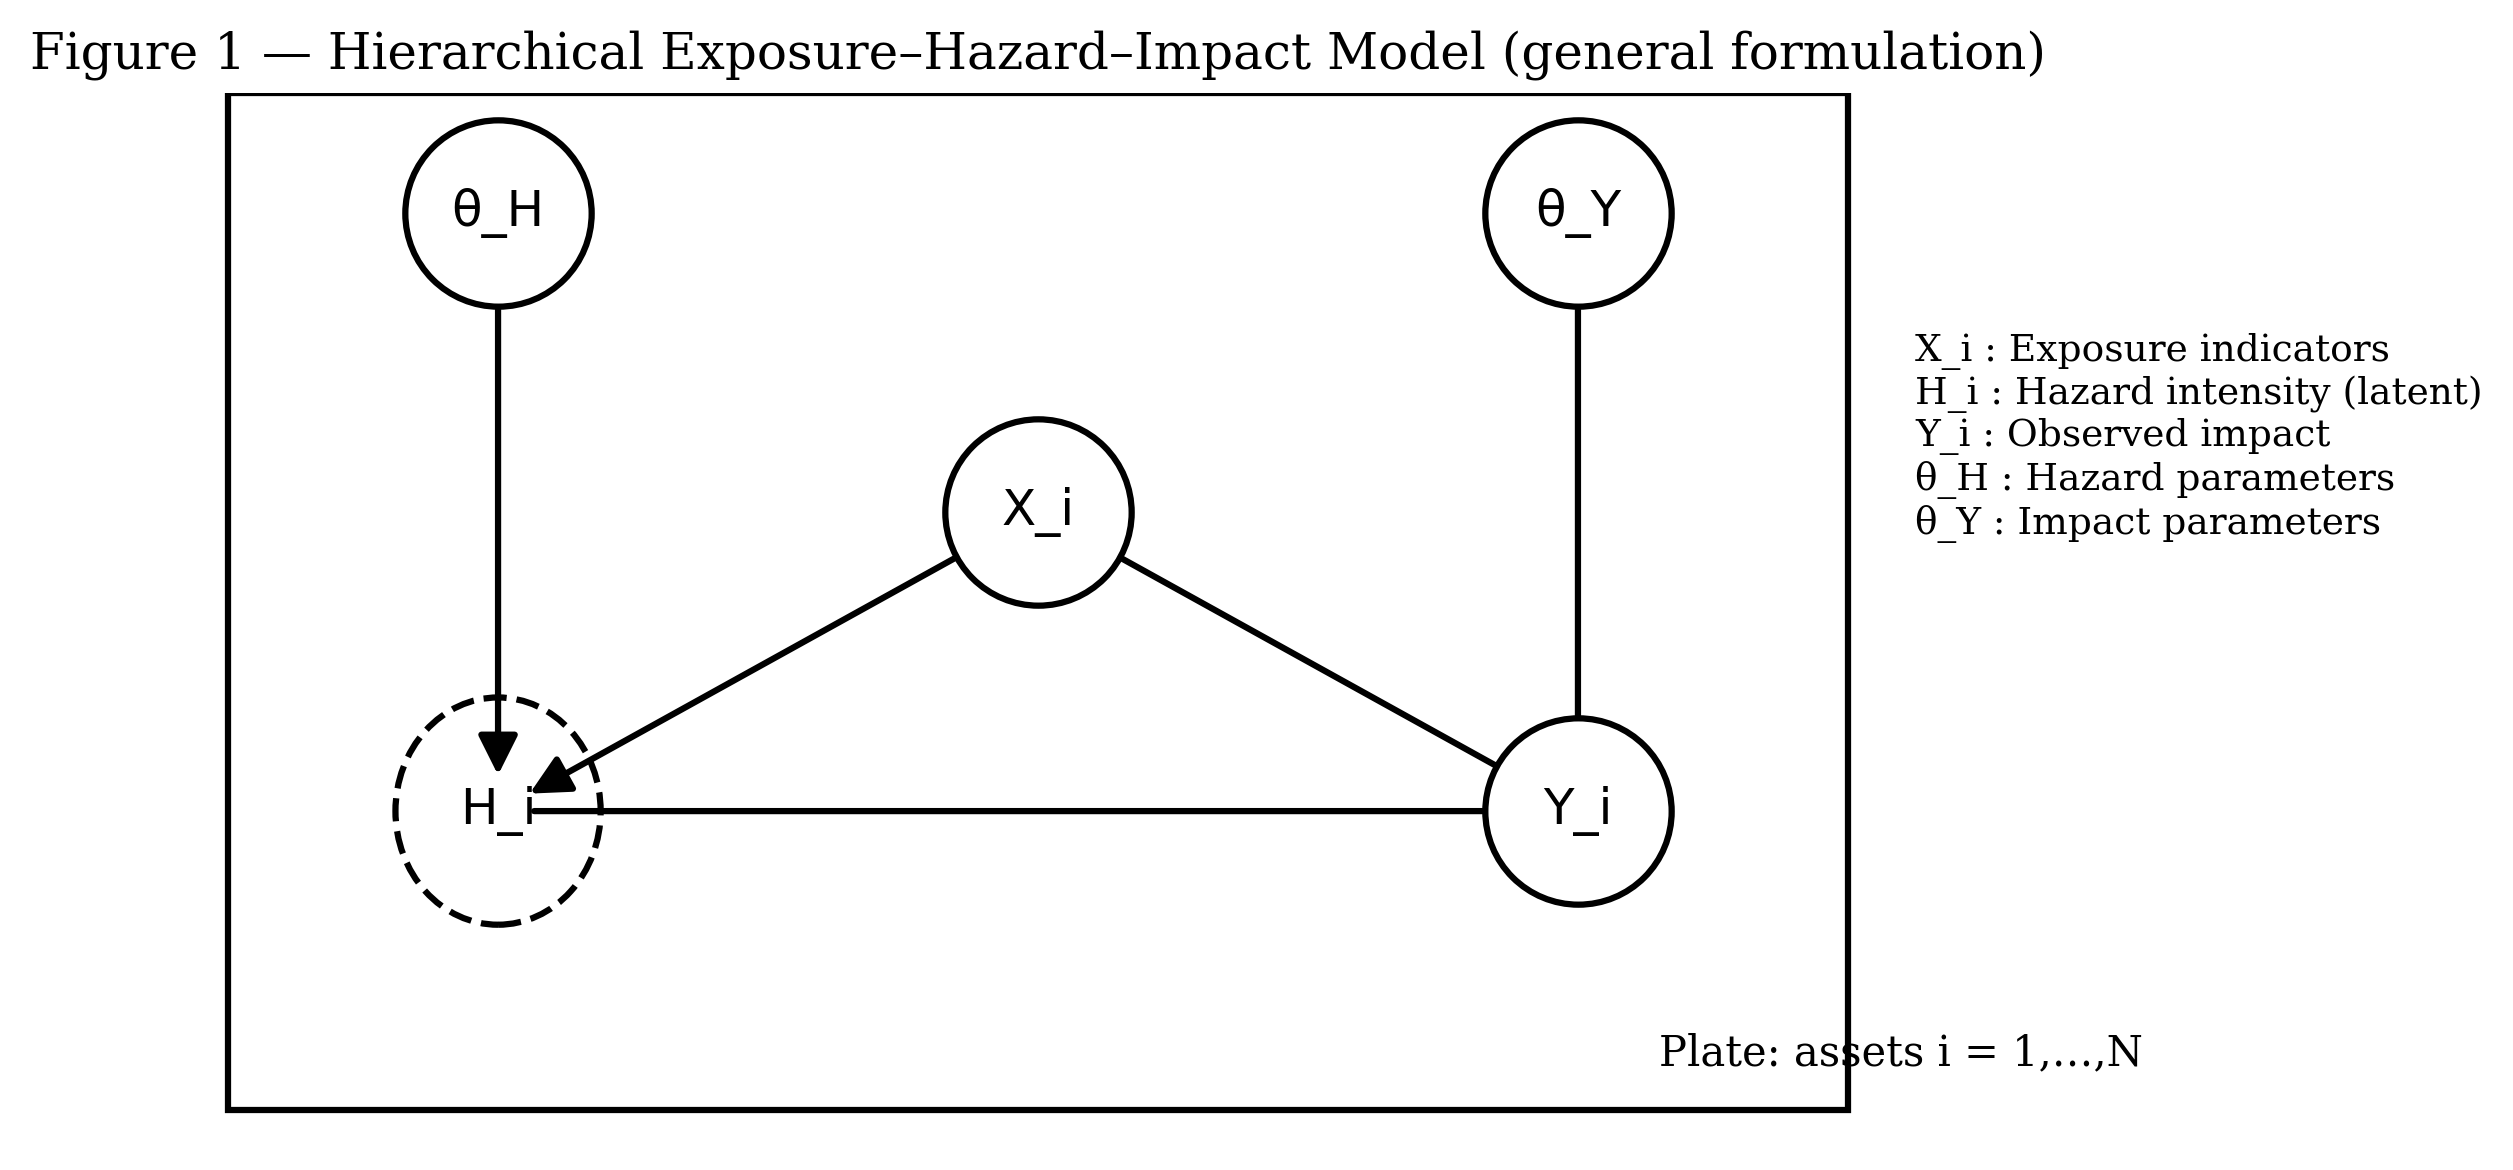
\includegraphics[keepaspectratio,alt={Hierarchical exposure--hazard--impact model}]{figures/fig01_graphical_model.png}}
\caption{Hierarchical exposure--hazard--impact model}
\end{figure}

Figure 1 illustrates the hierarchical exposure--hazard--impact structure
underlying the model.

\subsubsection{Decision stability
concept}\label{decision-stability-concept}

\begin{figure}
\centering
\pandocbounded{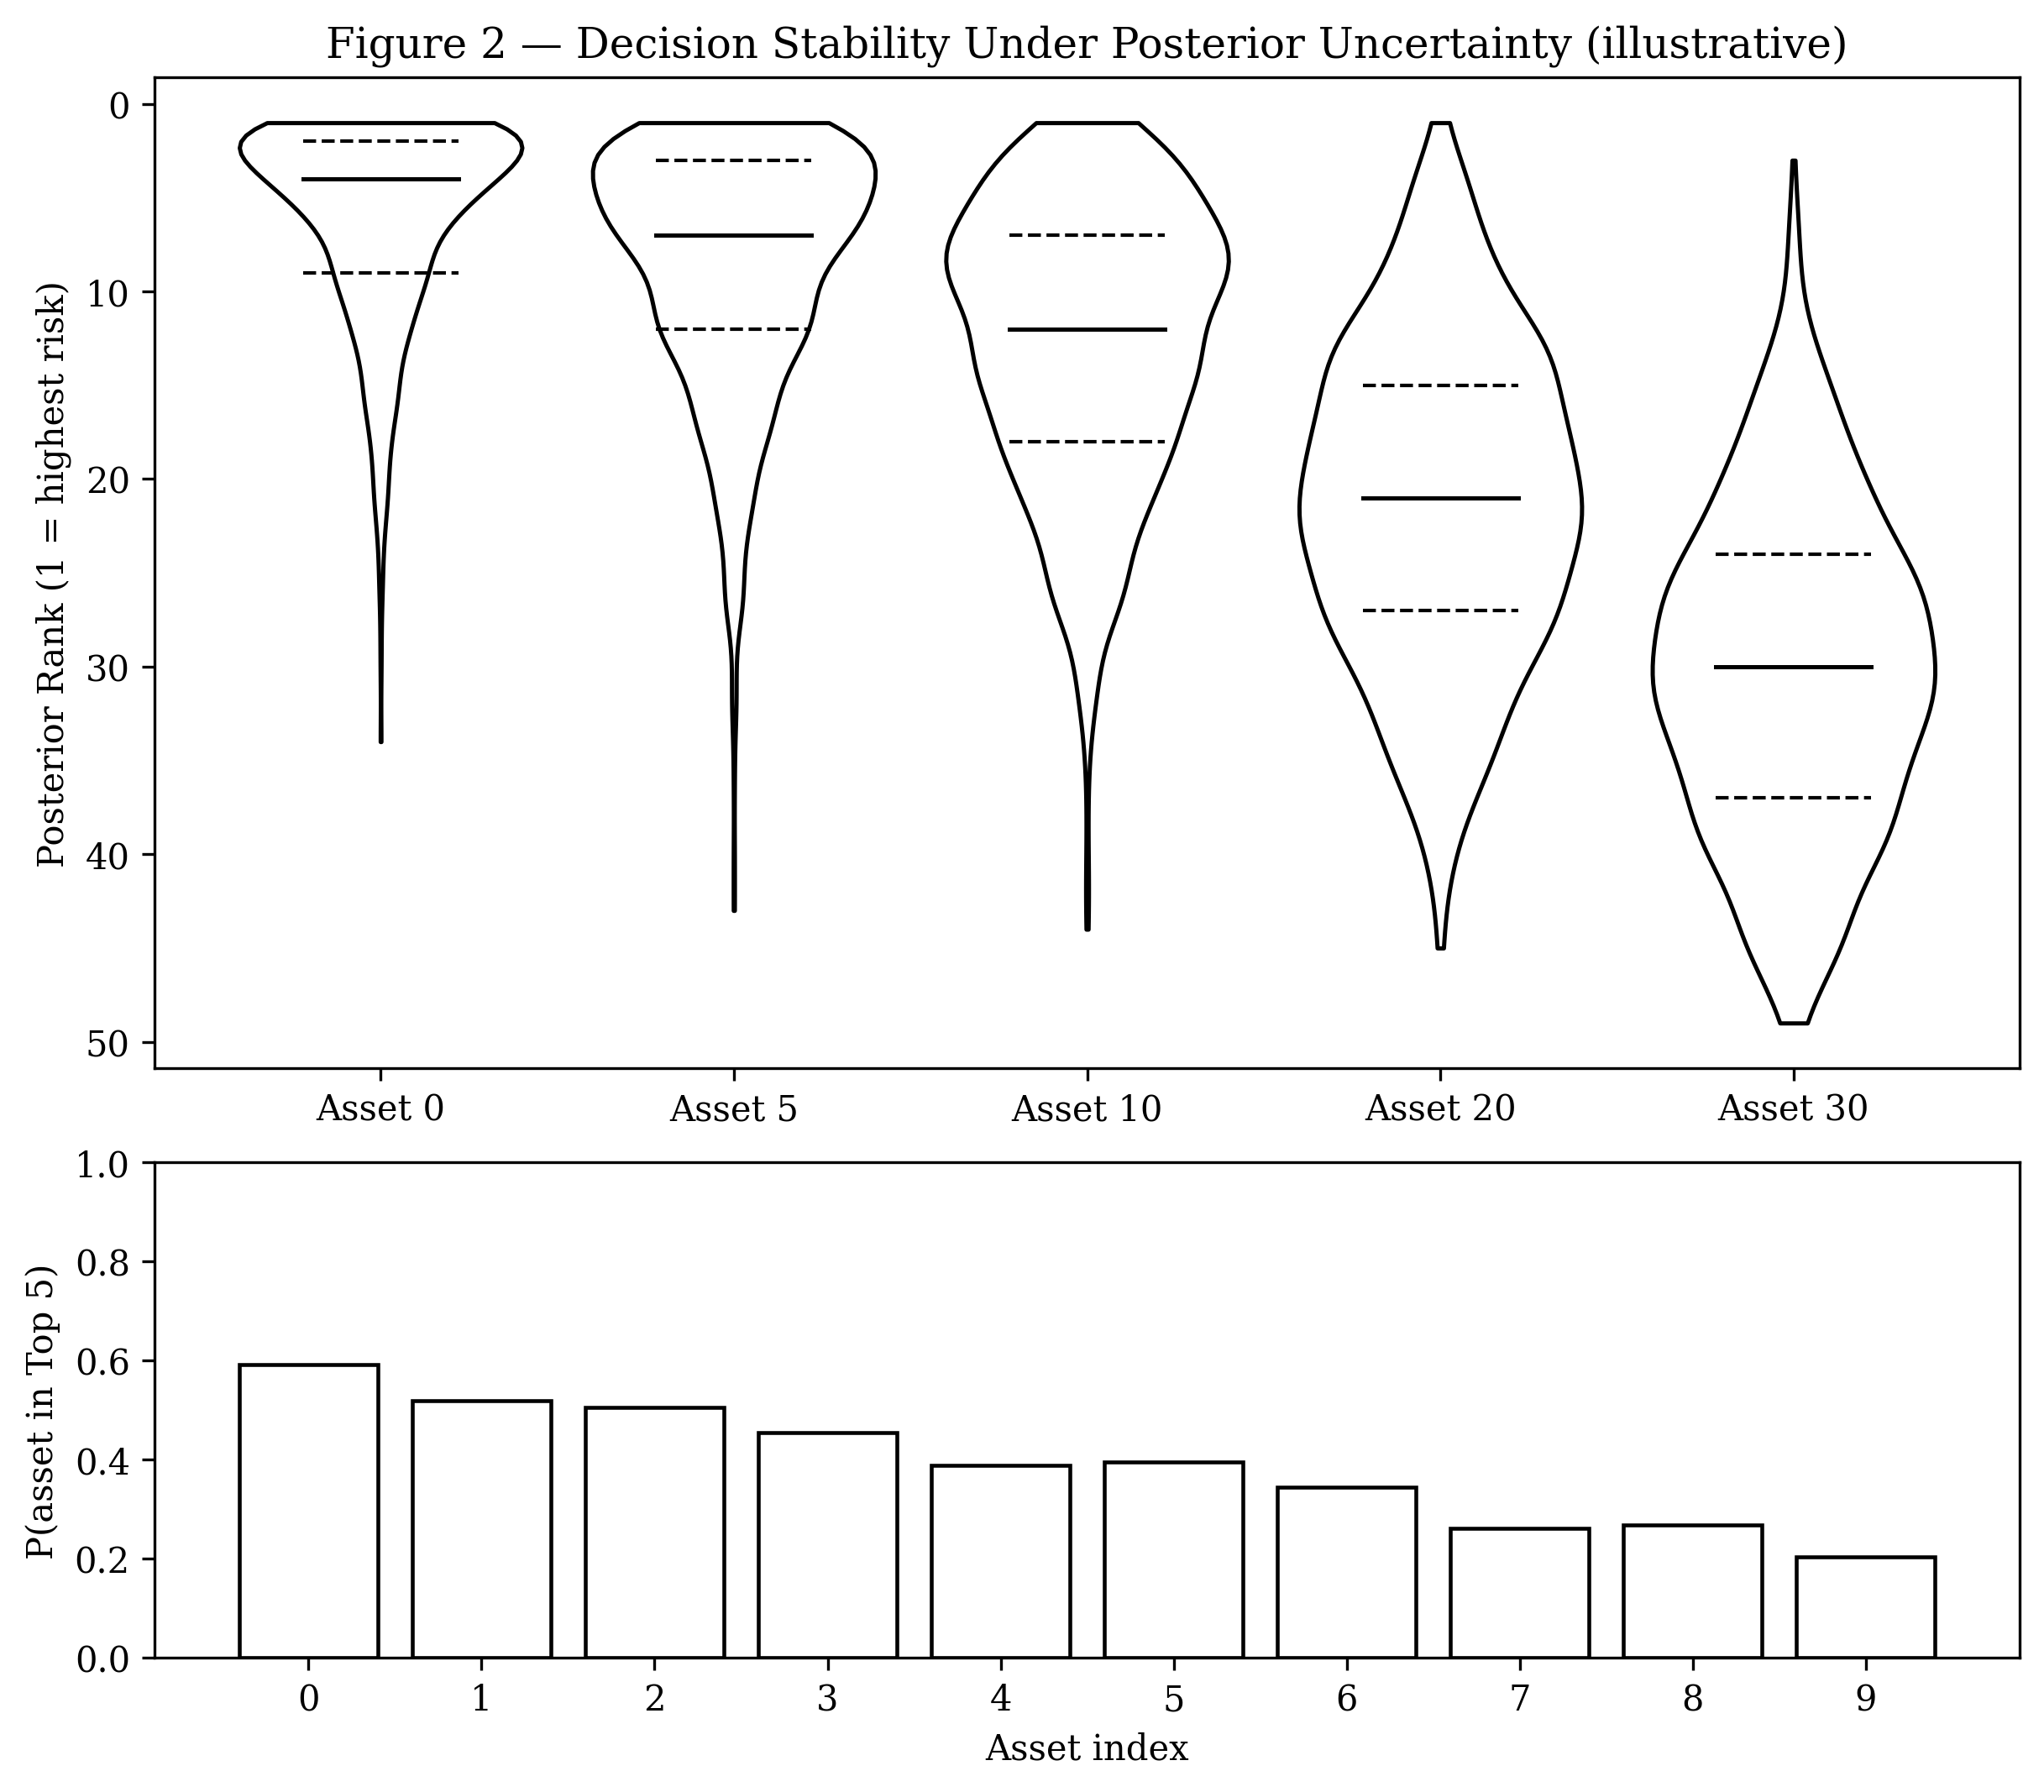
\includegraphics[keepaspectratio,alt={Decision stability concept}]{figures/fig02_decision_stability_concept.png}}
\caption{Decision stability concept}
\end{figure}

Figure 2 illustrates how posterior uncertainty propagates to asset
ranking distributions and top-k membership probabilities.

These quantities form the basis for the decision stability metrics
analysed in the Rotterdam case study.

\subsubsection{Domain-shift stress test
(conceptual)}\label{domain-shift-stress-test-conceptual}

\begin{figure}
\centering
\pandocbounded{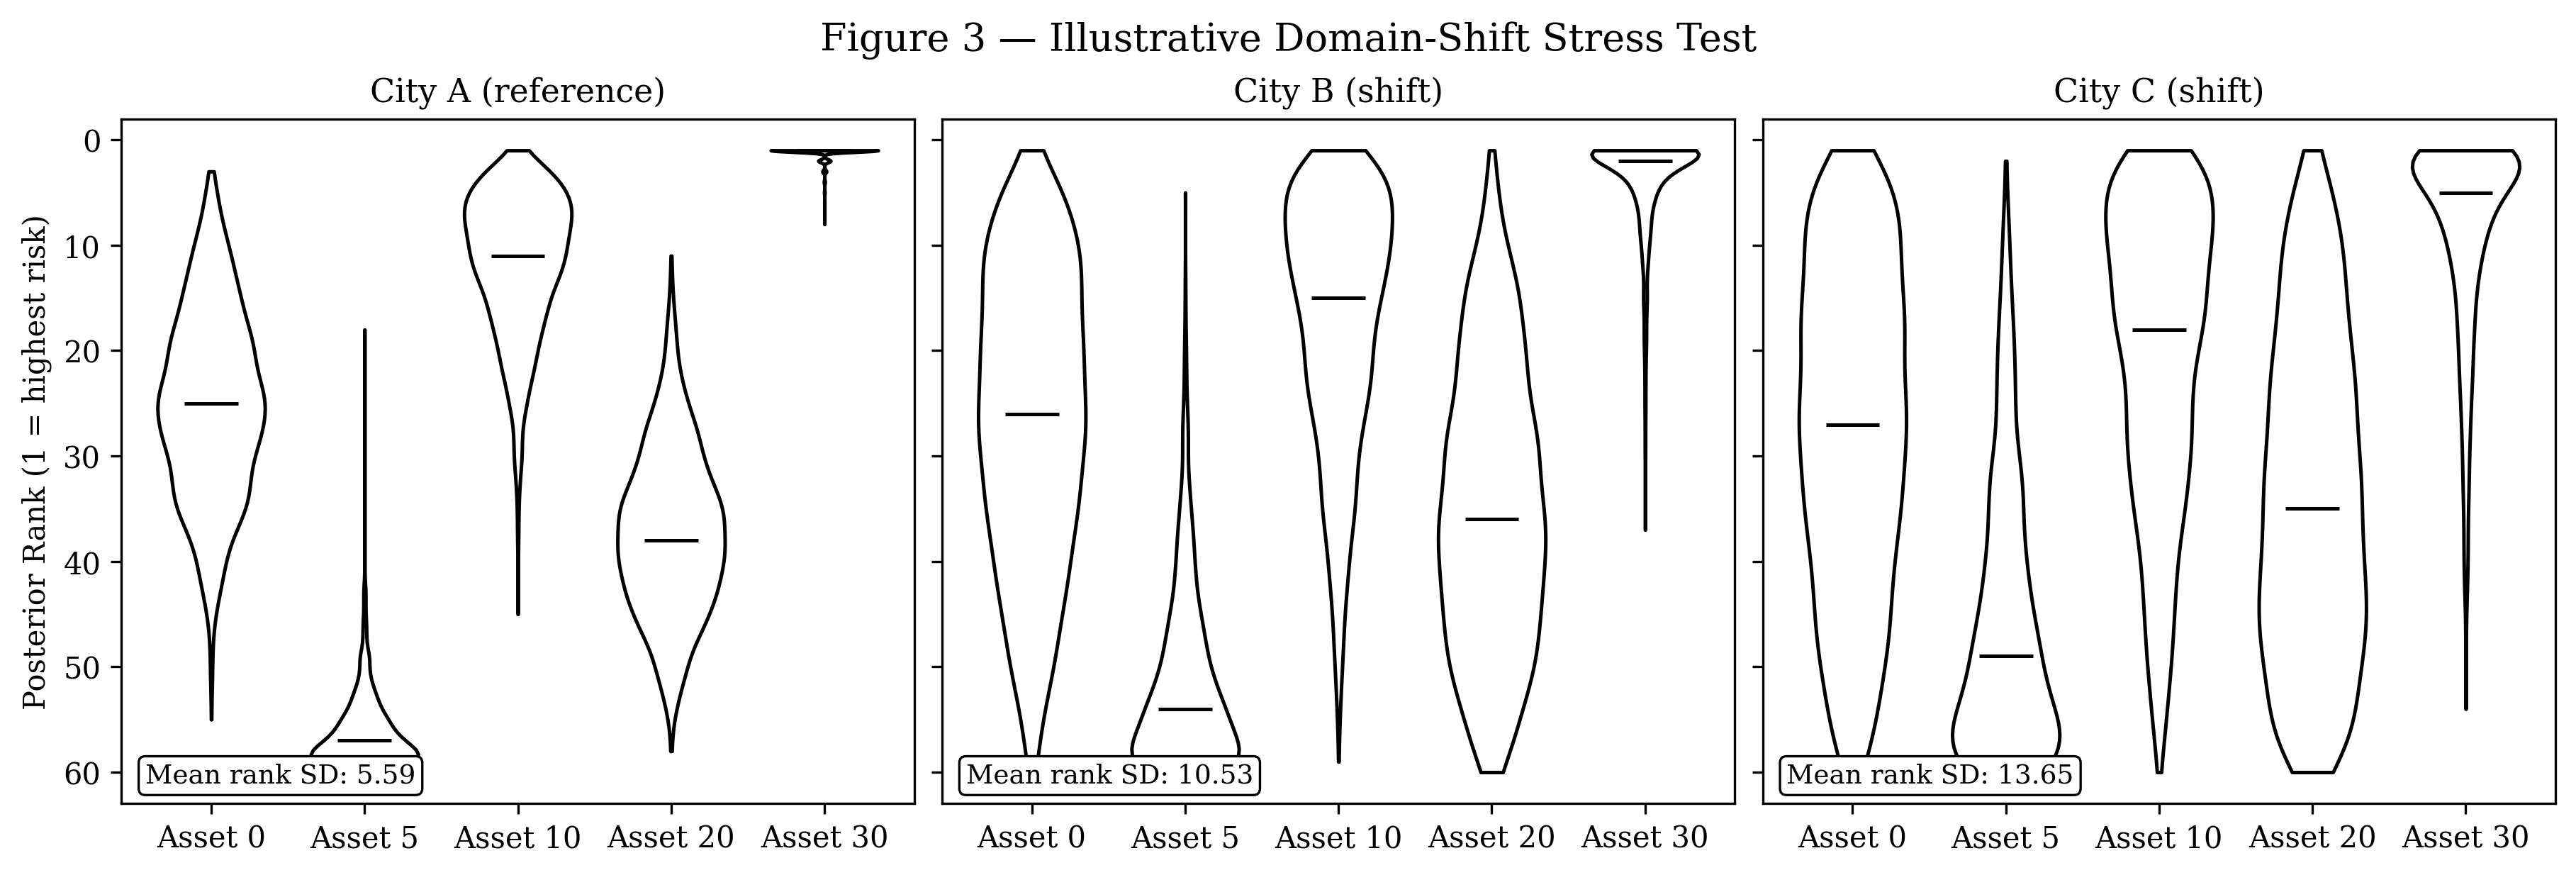
\includegraphics[keepaspectratio,alt={Domain-shift stress test concept}]{figures/fig03_domain_shift_illustrative.png}}
\caption{Domain-shift stress test concept}
\end{figure}

Figure 3 illustrates the conceptual domain-shift experiment proposed for
later phases of the research. The model specification remains fixed
while the framework is applied across different cities. If the
generative assumptions are stable, posterior ranking behaviour should
remain similar across cities. Under domain shift, ranking variability is
expected to increase, producing wider posterior rank distributions and
larger decision instability.

This experiment forms the basis of the cross-city transfer analysis
planned for future phases of the research.

\begin{center}\rule{0.5\linewidth}{0.5pt}\end{center}

\section{3. Data and Study Area}\label{data-and-study-area}

The modelling pipeline is applied to the municipality of
\textbf{Rotterdam, Netherlands}, containing approximately
\textbf{221,324 buildings}.

The dataset integrates several open data sources:

\begin{itemize}
\tightlist
\item
  \textbf{OpenStreetMap building footprints}
\item
  \textbf{Dutch hydrography datasets}
\item
  \textbf{ERA5-Land precipitation data}
\end{itemize}

\subsubsection{Exposure proxy}\label{exposure-proxy}

A deterministic exposure proxy \(\hat{E}_i\) is constructed using
spatial indicators of building proximity to water bodies and local
hydrographic density.

In Phase 1, exposure is represented by a deterministic index constructed
from hydrography proximity features, including distance to the nearest
water body and water length density within multiple buffer radii, and
standardised prior to modelling.

\subsubsection{Hazard proxy}\label{hazard-proxy}

A pluvial hazard proxy \(H_i\) is derived from precipitation forcing
indicators. The hazard representation is intentionally simplified in
Phase 1 to focus on validating the inference pipeline.

Hazard is represented by a deterministic pluvial forcing proxy derived
from ERA5-Land precipitation indicators and standardised prior to
modelling.

\subsubsection{Outcome variable}\label{outcome-variable}

The outcome variable represents a \textbf{synthetic damage indicator},
used solely to validate the probabilistic inference structure. No claims
of empirical calibration are made in this phase. The purpose of this
synthetic outcome is not to estimate real-world flood risk, but to
evaluate the behaviour of the probabilistic inference-to-decision
pipeline under controlled conditions.

\begin{center}\rule{0.5\linewidth}{0.5pt}\end{center}

\section{4. Bayesian Model}\label{bayesian-model}

The model defines a simple generative structure linking exposure, hazard
proxy, and binary impact outcome. We assume that, conditional on the
proxy variables \(E_i\) and \(H_i\), asset-level outcomes \(Y_i\) are
generated independently across assets according to a Bernoulli process
with probability \(p_i\). The variables \(E_i\) and \(H_i\) are treated
as observed proxies for latent exposure and hazard processes, and no
additional dependence structure is modelled at this stage.

Asset-level impact probability is modelled using a logistic regression
structure:

\[
p_i =
\text{logit}^{-1}
\left(
\alpha + \beta_E E_i + \beta_H H_i
\right)
\]

\[
Y_i \sim \text{Bernoulli}(p_i)
\]

where:

\begin{itemize}
\tightlist
\item
  \(E_i\) denotes the exposure proxy
\item
  \(H_i\) denotes the hazard proxy
\item
  \(Y_i \in \{0,1\}\) denotes the impact indicator
\end{itemize}

\subsubsection{Priors}\label{priors}

Weakly informative priors are assigned to model parameters:

\[
\alpha, \beta_E, \beta_H \sim \mathcal{N}(0, 2.5)
\]

\subsubsection{Inference}\label{inference}

Posterior inference is performed using \textbf{PyMC} with Hamiltonian
Monte Carlo sampling.

Diagnostics include:

\begin{itemize}
\tightlist
\item
  \(\hat{R}\) convergence diagnostics
\item
  effective sample size (ESS)
\item
  posterior predictive checks
\end{itemize}

All model parameters achieved \(\hat{R} < 1.01\), with effective sample
sizes exceeding 500 for all reported variables, indicating stable and
well-mixed posterior sampling.

Posterior draws produce asset-level probability distributions of impact.

We sample using NUTS in PyMC with 2 chains, 500 tuning steps and 500
posterior draws per chain (\texttt{target\_accept\ =\ 0.9}). Citywide
decision metrics are computed by applying posterior draws to the full
building set (\(N = 221{,}324\)).

\subsubsection{Model scope}\label{model-scope}

The logistic specification is intentionally minimal, serving as a
baseline to isolate the behaviour of posterior-derived decision metrics
rather than to optimise predictive performance. The objective in Phase 1
is to validate the probabilistic inference and decision pipeline, not to
provide a fully calibrated predictive model.

\subsubsection{Posterior distribution}\label{posterior-distribution}

The posterior distribution over model parameters is

\[
p(\theta \mid \text{data})
\propto
p(\text{data} \mid \theta)\,p(\theta)
\]

where

\[
\theta = (\alpha, \beta_E, \beta_H)
\]

\begin{center}\rule{0.5\linewidth}{0.5pt}\end{center}

\section{5. Posterior-Derived Decision
Metrics}\label{posterior-derived-decision-metrics}

Rather than relying on point estimates, prioritisation decisions are
derived from posterior draws.

\subsubsection{Posterior mean risk}\label{posterior-mean-risk}

For each asset \(i\):

\[
p_{\text{mean}, i}
=
\mathbb{E}_{p(\theta \mid \text{data})}
\left[
P(Y_i = 1 \mid \theta)
\right]
\]

The distribution of posterior mean probabilities across the city is
analysed in the Results section.

\subsubsection{Top-k membership
probability}\label{top-k-membership-probability}

For a prioritisation threshold \(k\), the probability that asset \(i\)
belongs to the top-k highest risk assets is:

\[
P(i \in \text{Top}_k \mid \text{posterior})
\]

\subsubsection{Decision stability
metrics}\label{decision-stability-metrics}

Several metrics quantify ranking stability:

\begin{itemize}
\tightlist
\item
  \textbf{Top-k overlap ratio}
\item
  \textbf{Posterior entropy of membership probability}
\item
  \textbf{Borderline share}, defined as assets with
\end{itemize}

\[
0.2 < P(i \in \text{Top}_k) < 0.8
\]

\subsubsection{Computational
implementation}\label{computational-implementation}

All analyses are implemented in Python using PyMC for Bayesian inference
and ArviZ for posterior diagnostics. The analysis pipeline, data
preparation scripts, and manuscript sources are available in open
repositories to support reproducibility.

\begin{center}\rule{0.5\linewidth}{0.5pt}\end{center}

\section{6. Results}\label{results}

The analysis covers \textbf{221,324 buildings} across the municipality
of Rotterdam.

\subsection{6.1 Posterior risk
distribution}\label{posterior-risk-distribution}

Figure 4 shows the empirical cumulative distribution of posterior mean
impact probabilities across all buildings.

\begin{figure}
\centering
\pandocbounded{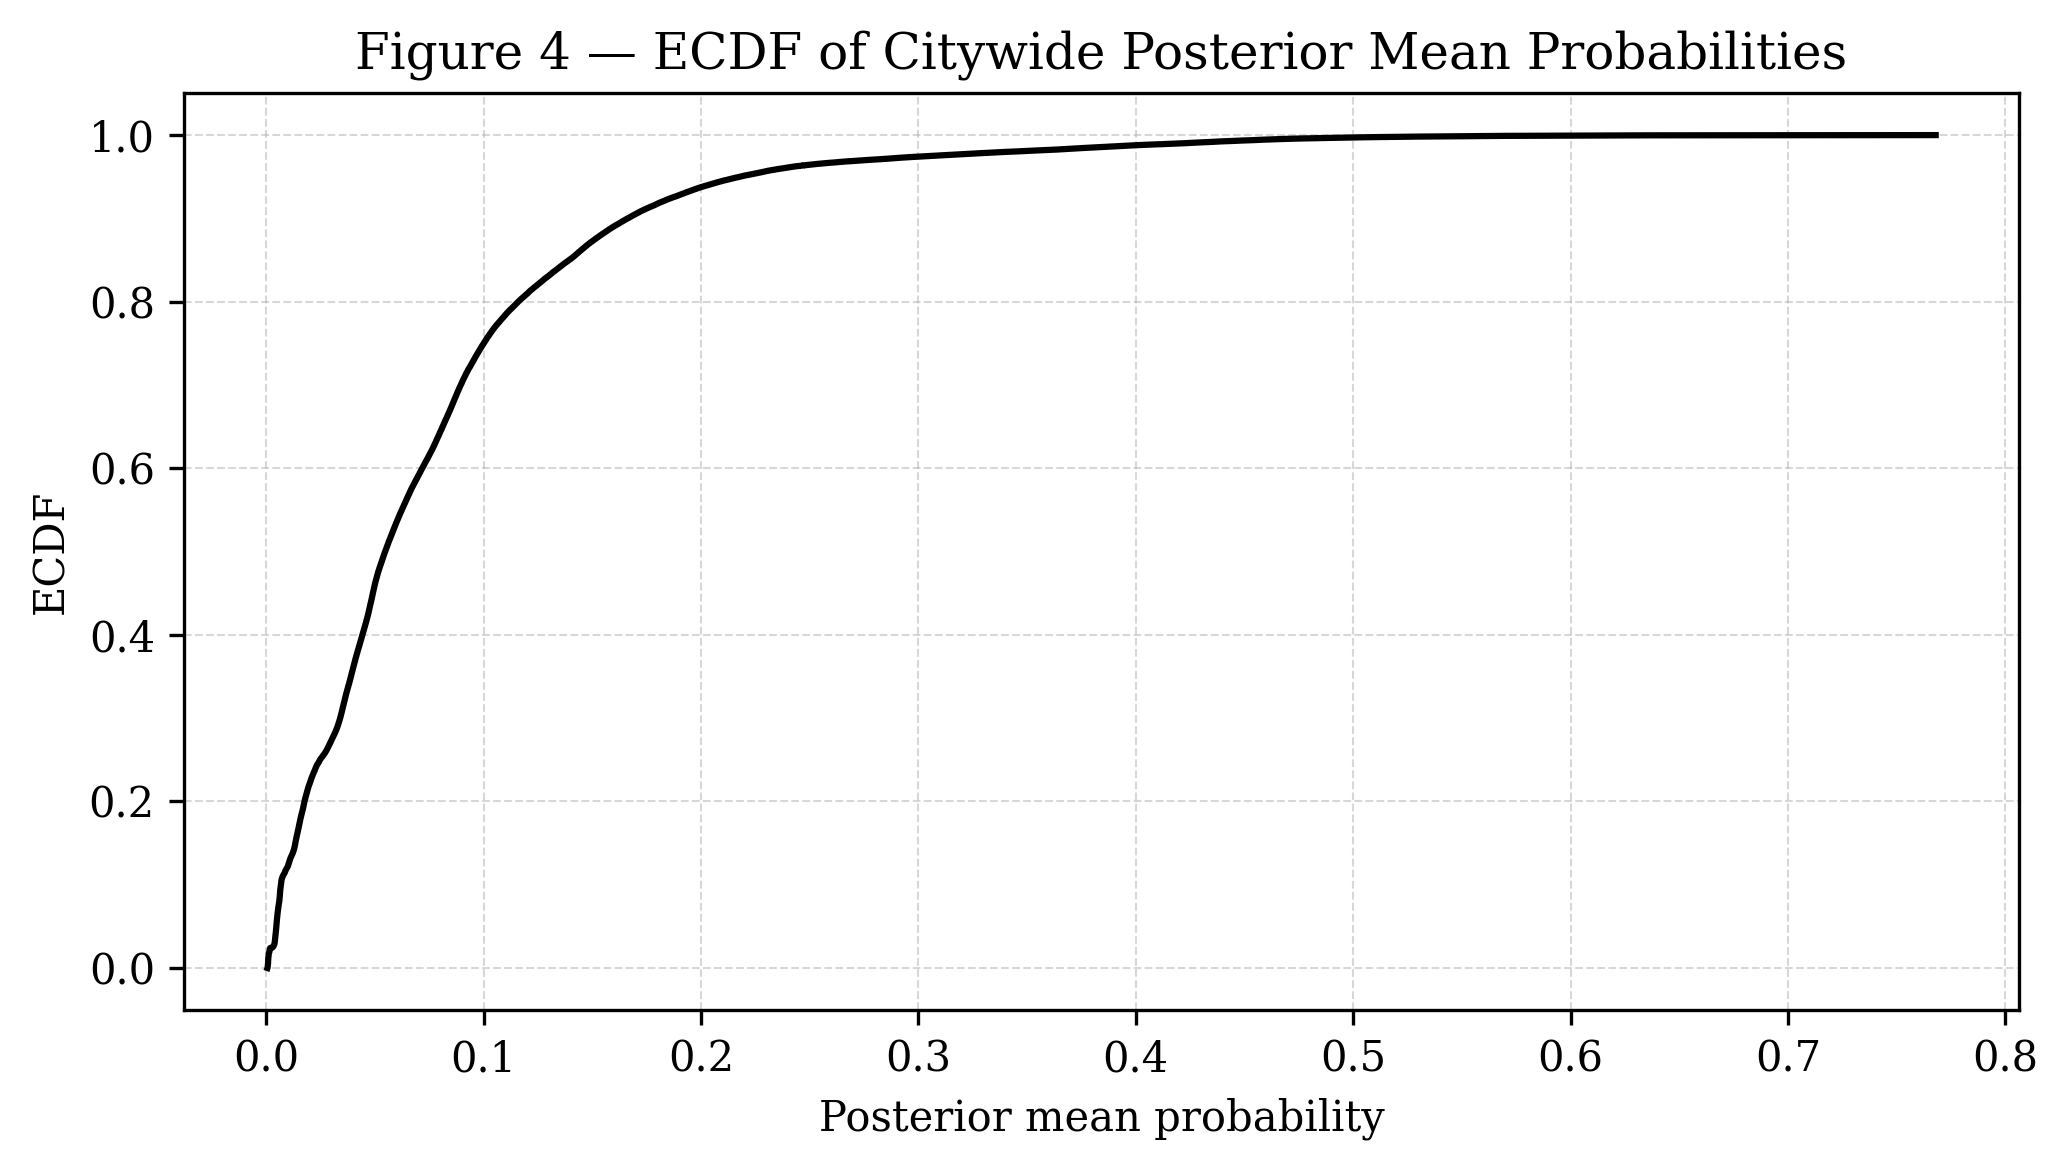
\includegraphics[keepaspectratio,alt={Empirical cumulative distribution of posterior mean probabilities}]{figures/fig04_pmean_city_ecdf.png}}
\caption{Empirical cumulative distribution of posterior mean
probabilities}
\end{figure}

Posterior mean probabilities are strongly concentrated near low values,
with a \textbf{mean of 0.077}, a \textbf{median of 0.055}, and a
\textbf{90th percentile of 0.166}. Only a small fraction of assets
occupy the upper tail of the distribution, with the \textbf{99th
percentile reaching 0.421} and a maximum value of \textbf{0.768}.

This skewed distribution reflects the sparse structure of the synthetic
outcome generation process and provides a useful setting for analysing
how posterior uncertainty affects prioritisation decisions.

\subsection{6.2 Decision stability across prioritisation
thresholds}\label{decision-stability-across-prioritisation-thresholds}

Decision stability is evaluated by analysing how frequently assets fall
within the top-k highest risk positions across posterior draws.

\begin{figure}
\centering
\pandocbounded{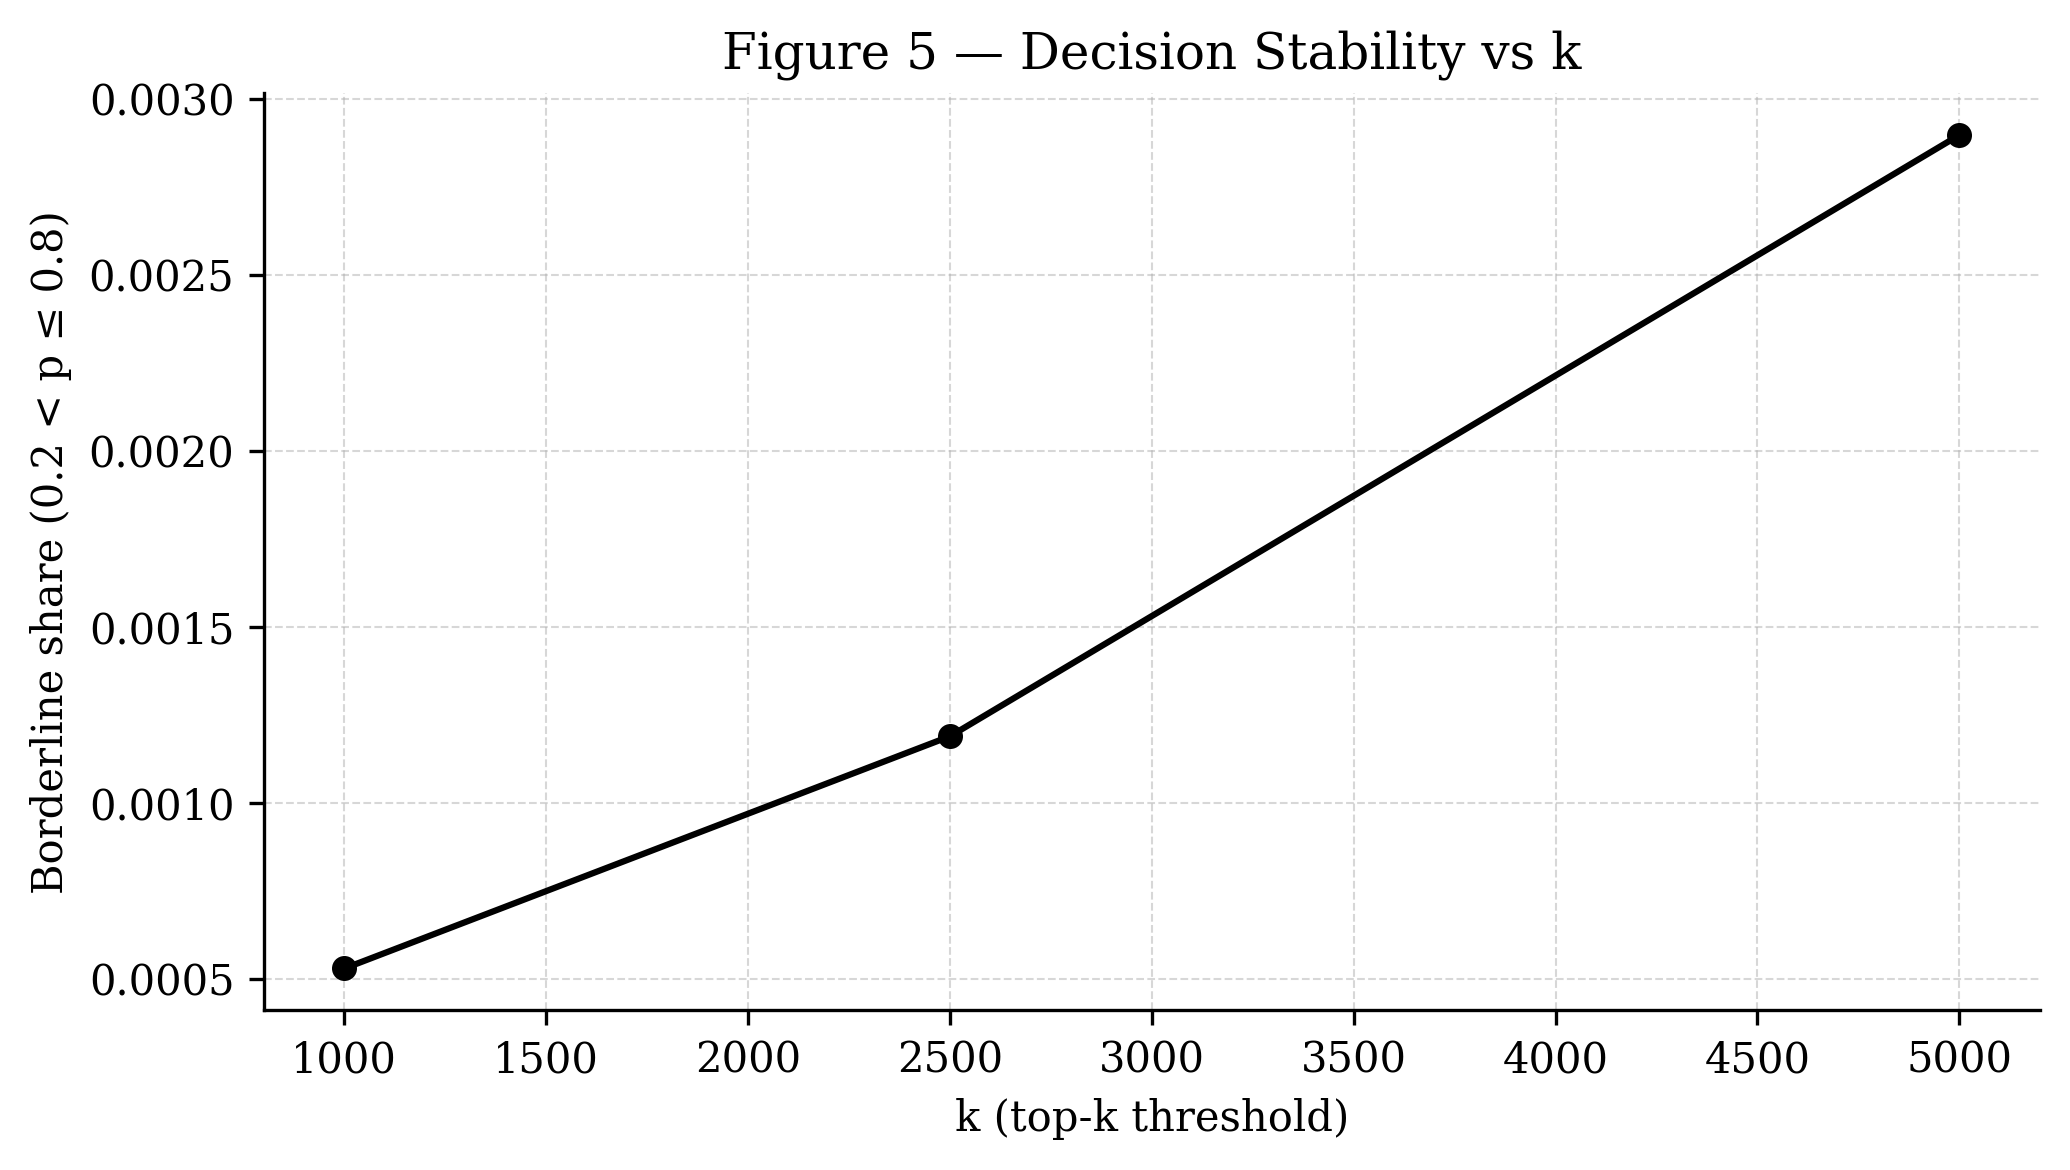
\includegraphics[keepaspectratio,alt={Borderline share across prioritisation thresholds}]{figures/fig05_borderline_vs_k.png}}
\caption{Borderline share across prioritisation thresholds}
\end{figure}

The borderline share represents assets whose top-k membership
probability lies between 0.2 and 0.8. These assets occupy the decision
boundary where prioritisation outcomes are sensitive to posterior
uncertainty.

Across prioritisation thresholds, the borderline share remains extremely
small relative to the total asset population. For \textbf{k = 1000}, the
borderline share is \textbf{0.053\%}, increasing slightly to
\textbf{0.29\%} for \textbf{k = 5000}. Even at larger prioritisation
sets, only a very small subset of assets exhibits unstable
prioritisation behaviour.

This indicates that posterior uncertainty affects only a narrow decision
boundary rather than the overall prioritisation structure.

\subsection{6.3 Borderline decision
region}\label{borderline-decision-region}

To better understand where instability occurs, we examine the
distribution of top-k membership probabilities across assets.

\begin{figure}
\centering
\pandocbounded{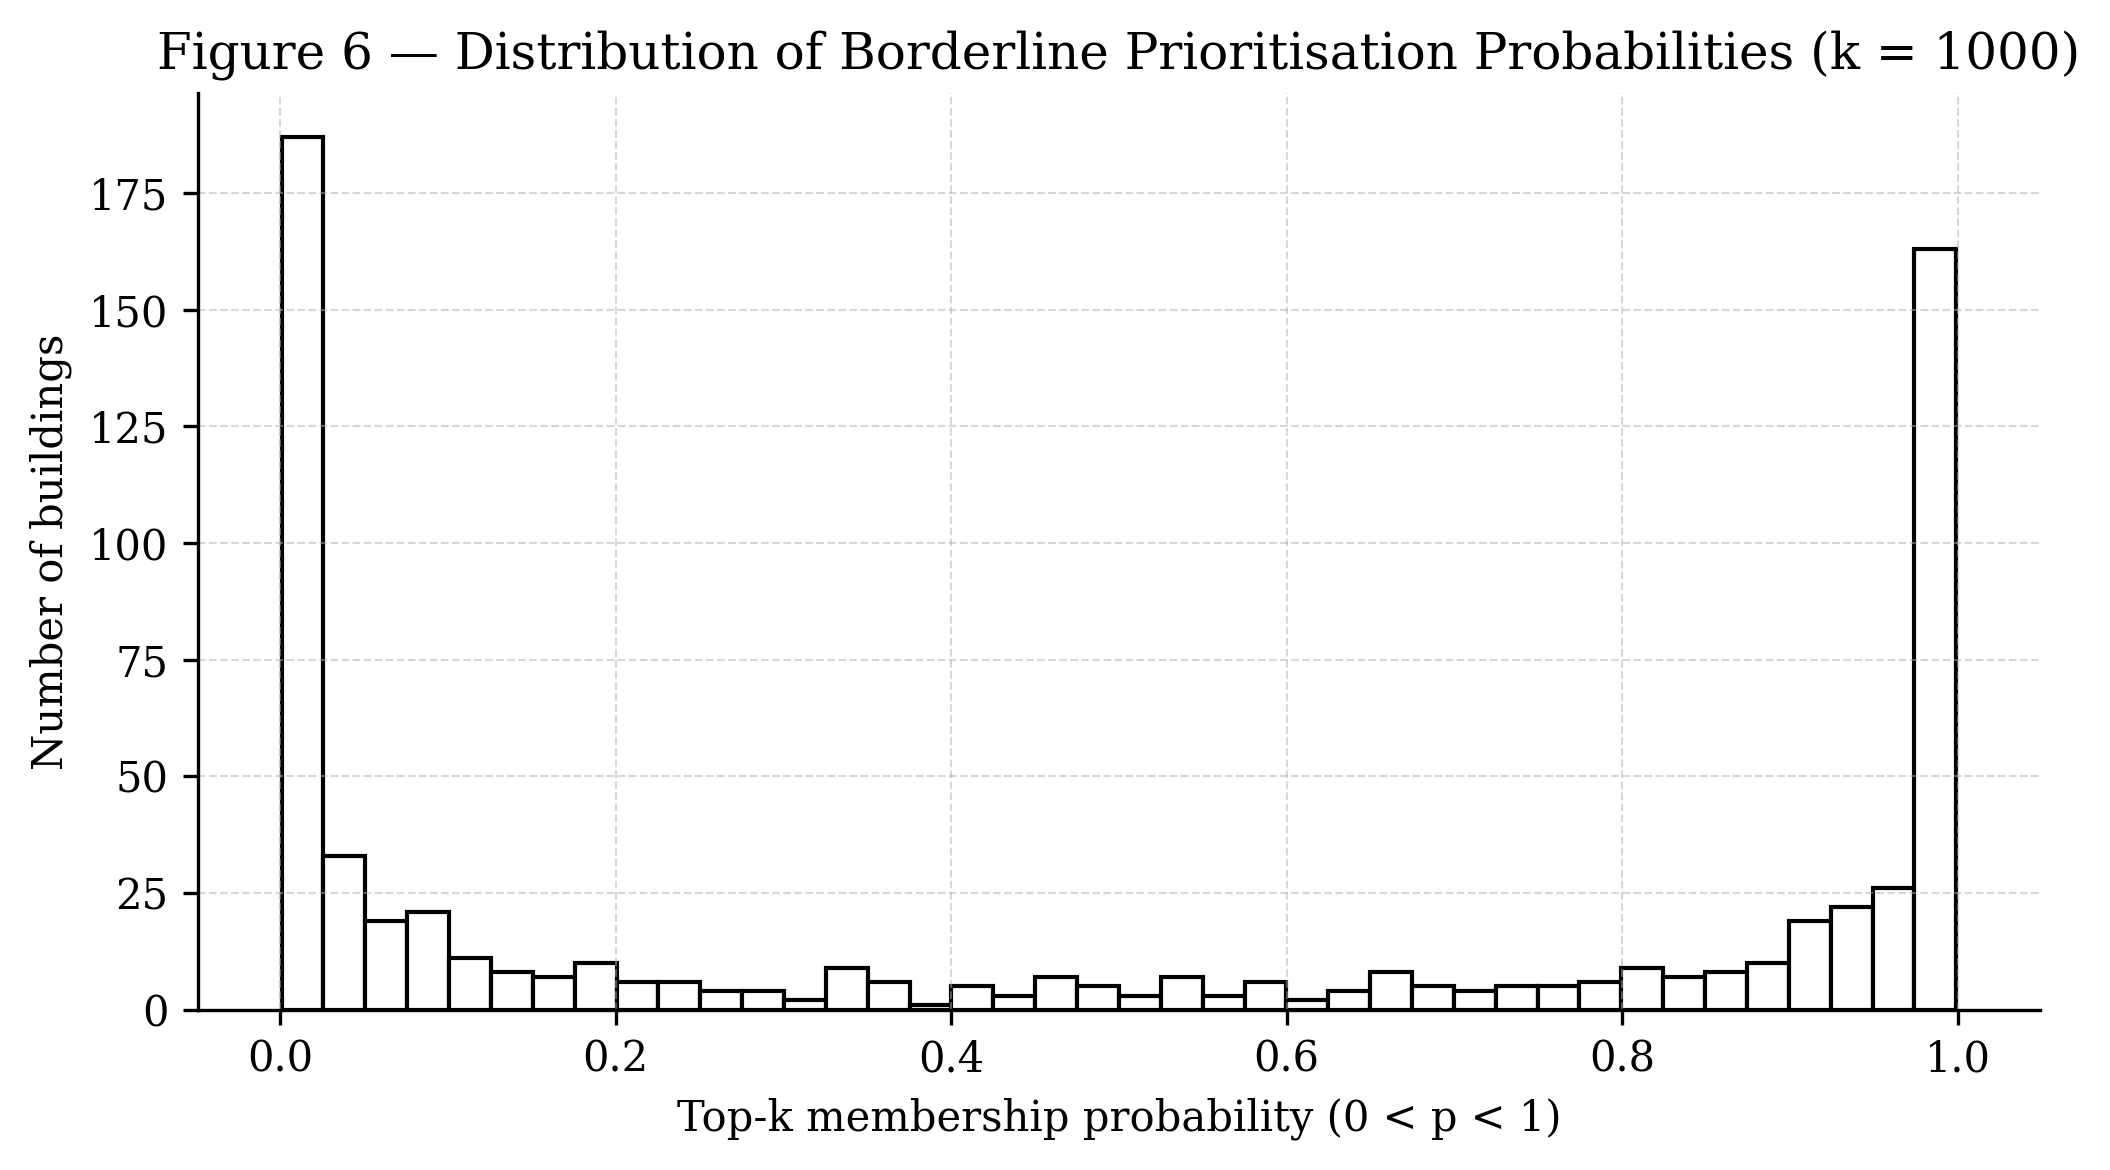
\includegraphics[keepaspectratio,alt={Distribution of top-k membership probabilities}]{figures/fig06_topk_prob_histogram.png}}
\caption{Distribution of top-k membership probabilities}
\end{figure}

For the \textbf{Top-1000 prioritisation threshold}, the mean membership
probability is \textbf{0.0045}, consistent with the expected proportion
of selected assets in the citywide dataset. Most assets have membership
probabilities close to either \textbf{0} or \textbf{1}, indicating
stable prioritisation outcomes.

Only a very small fraction of assets fall within the intermediate region
\(0.2 < P(i \in \text{Top}_k) < 0.8\), with a borderline share of
approximately \textbf{0.00052}. These assets form a narrow decision
boundary where ranking positions fluctuate across posterior draws and
where additional information or improved modelling could most influence
prioritisation decisions.

Overall, posterior uncertainty is not diffuse across the system but
sharply concentrated at the prioritisation boundary. Most assets exhibit
stable rankings, while only a small subset drives decision instability.
This suggests that probabilistic prioritisation is not only descriptive,
but operationally useful: it identifies exactly where additional data or
model refinement would have the greatest impact on decision quality.

This concentration of instability at the decision boundary implies that
most prioritisation decisions are robust under current assumptions, and
that uncertainty reduction efforts can be targeted efficiently rather
than applied uniformly across all assets.

\subsection{6.4 Robustness to Hazard
Perturbation}\label{robustness-to-hazard-perturbation}

The results above are derived using a deterministic hazard proxy. To
assess whether the observed concentration of decision instability
depends on this assumption, we introduce controlled perturbations to the
hazard representation. This experiment can be interpreted as a test of
whether the observed concentration of decision instability is an
artefact of deterministic hazard specification or a structural property
of the inference--decision pipeline.

The following values are computed on the inference subsample (N = 5000)
and are therefore not directly comparable to the citywide percentages
reported in Sections 6.2--6.3.

The standardised hazard variable is perturbed as:

\[
H_i^{\text{perturbed}} = H_i + \epsilon_i, \quad \epsilon_i \sim \mathcal{N}(0, \sigma)
\]

We evaluate multiple perturbation levels:

\begin{itemize}
\tightlist
\item
  \(\sigma\) = 0.00 (baseline)
\item
  \(\sigma\) = 0.05
\item
  \(\sigma\) = 0.10
\item
  \(\sigma\) = 0.20
\item
  \(\sigma\) = 0.30
\end{itemize}

For each scenario, the full inference pipeline is re-run and decision
metrics are recomputed.

\subsubsection{Results}\label{results-1}

{\def\LTcaptype{none} % do not increment counter
\begin{longtable}[]{@{}ll@{}}
\toprule\noalign{}
\(\sigma\) & Borderline Share \\
\midrule\noalign{}
\endhead
\bottomrule\noalign{}
\endlastfoot
0.00 & 0.0158 \\
0.05 & 0.0130 \\
0.10 & 0.0148 \\
0.20 & 0.0172 \\
0.30 & 0.0174 \\
\end{longtable}
}

\begin{figure}
\centering
\pandocbounded{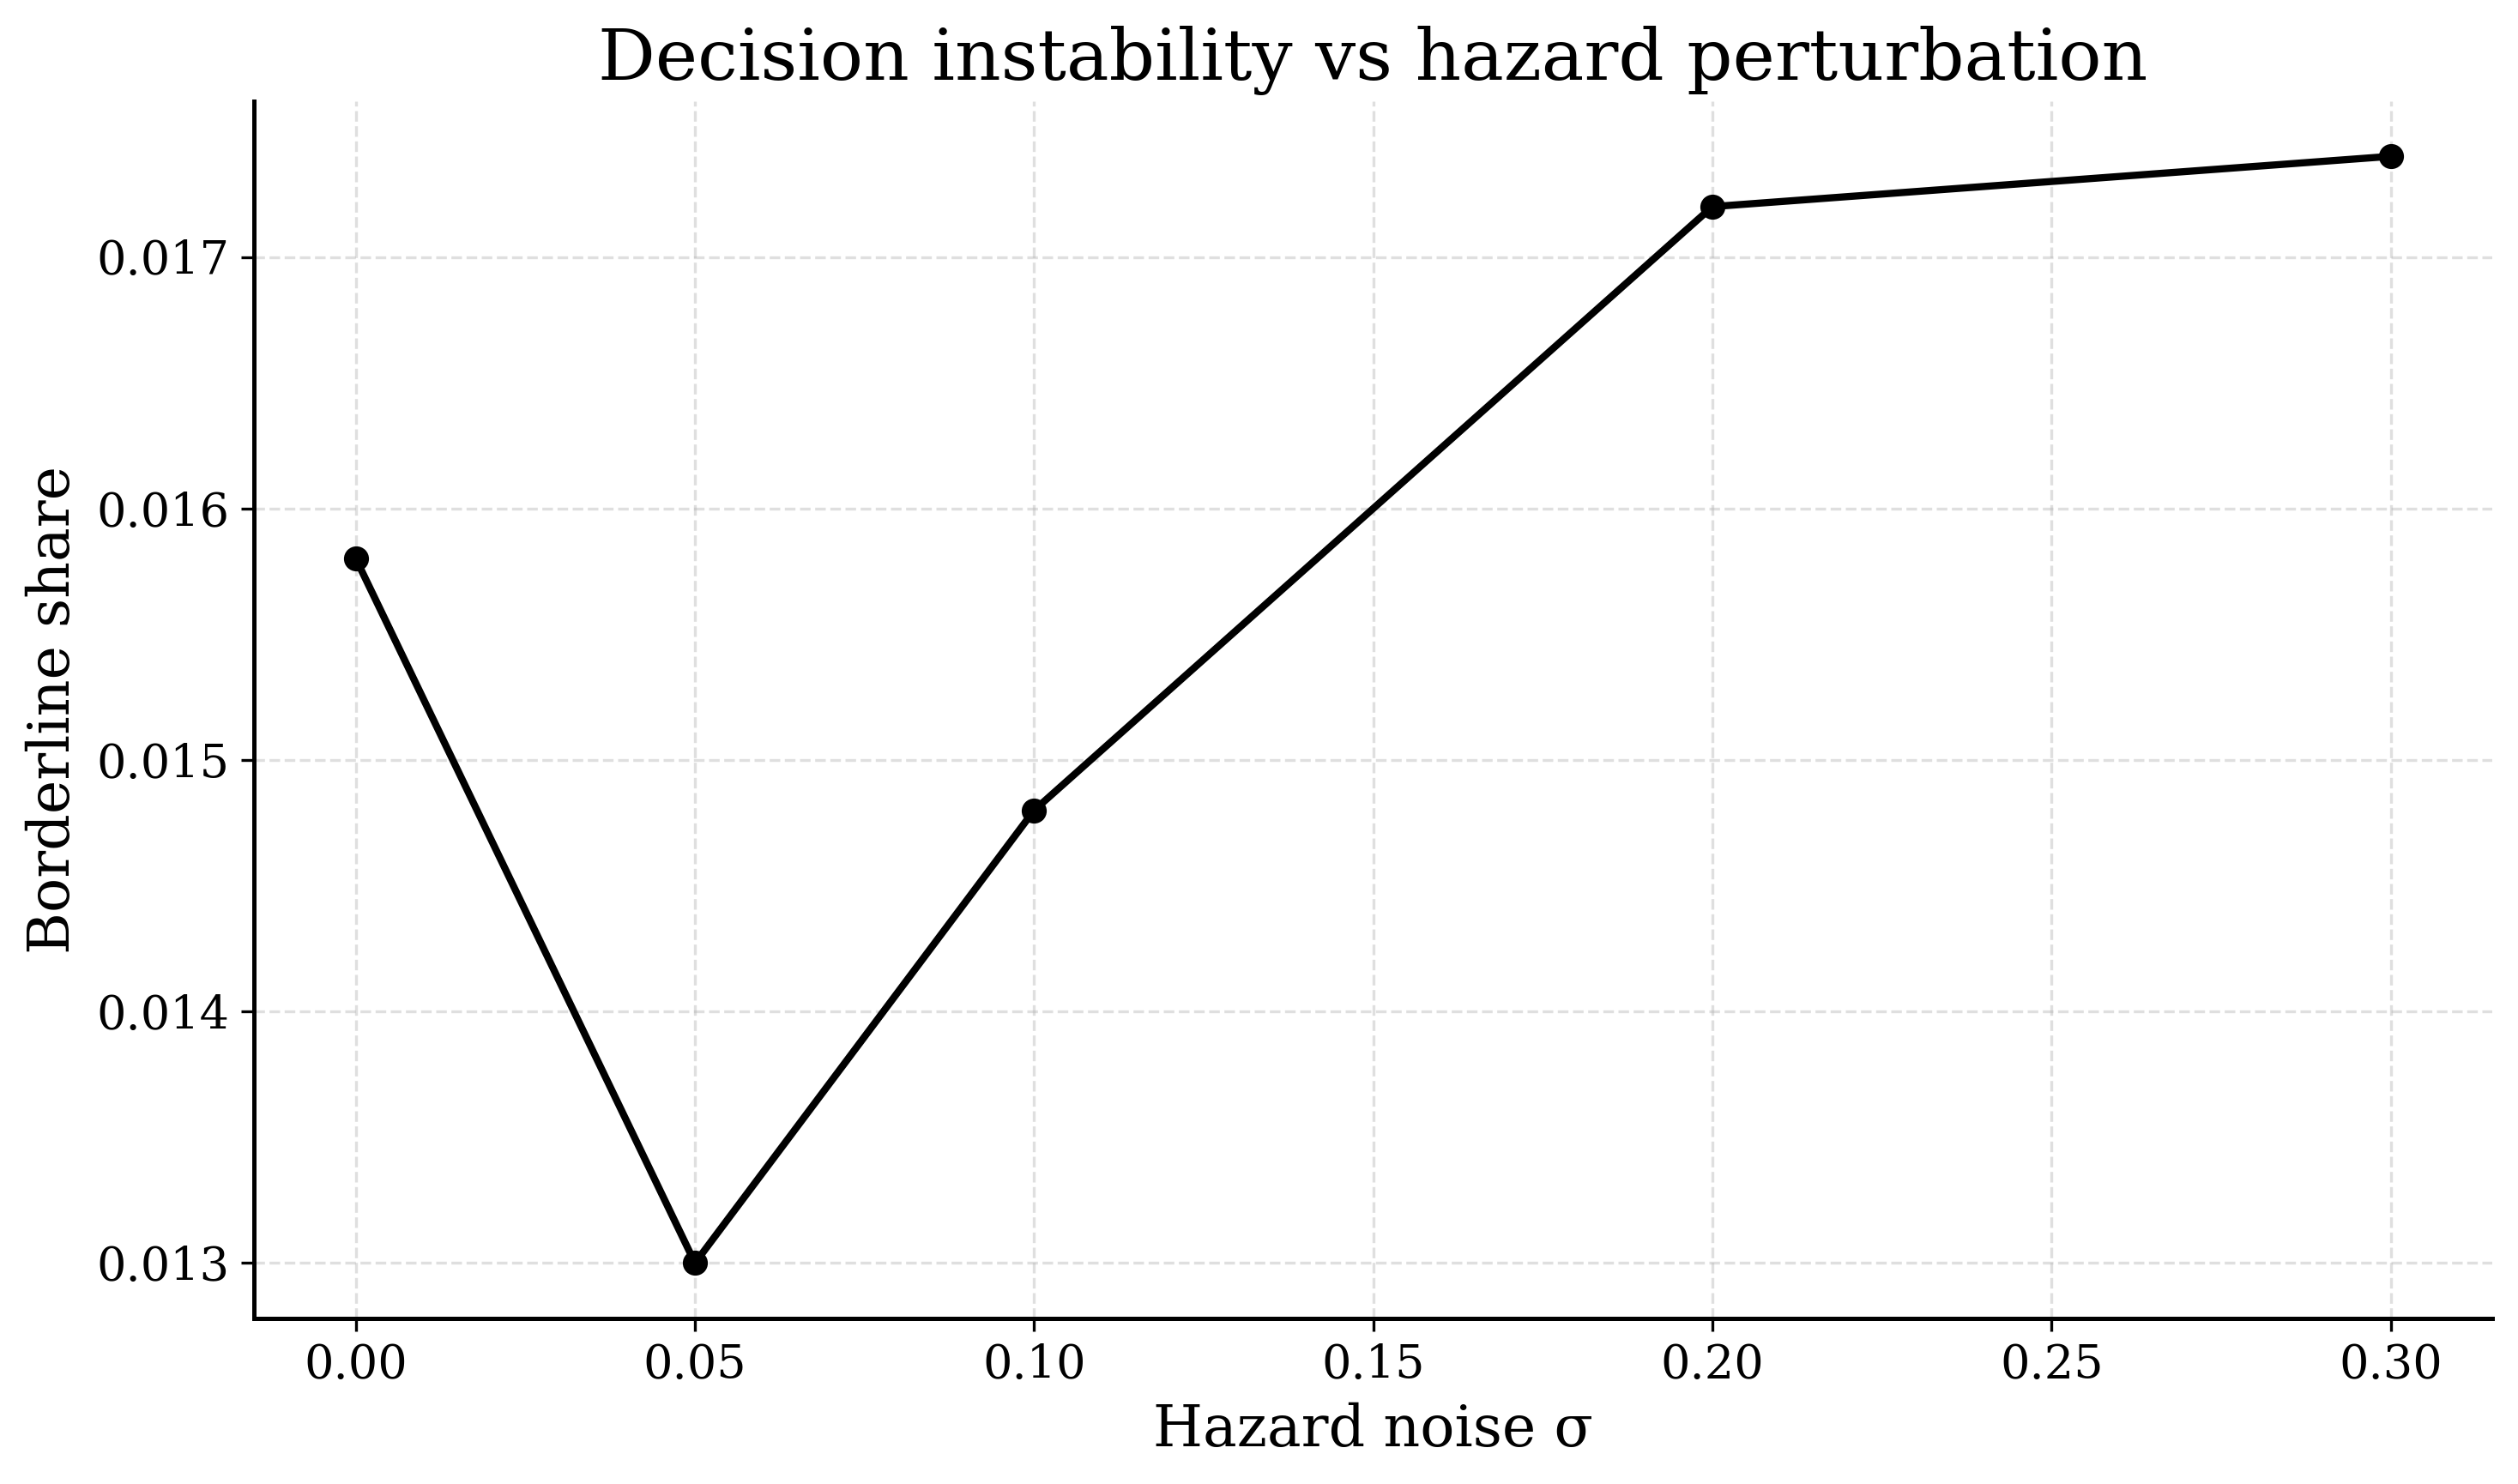
\includegraphics[keepaspectratio,alt={Decision instability vs hazard perturbation}]{figures/fig07_borderline_vs_sigma.png}}
\caption{Decision instability vs hazard perturbation}
\end{figure}

The borderline share remains within a narrow range
(\textasciitilde1.3--1.7\%) across all perturbation levels.

\subsubsection{Interpretation}\label{interpretation}

The concentration of decision instability within a narrow boundary is
robust to moderate perturbations (\(\sigma\) up to 0.30 in standardised
hazard space) of the hazard proxy.

This indicates that the observed prioritisation structure is not an
artefact of a fixed hazard input, but rather a structural property of
the model and data. Most assets retain stable prioritisation behaviour,
while a small subset near the decision threshold continues to drive
variability.

These results support the interpretation that posterior-derived
prioritisation stability is inherently localised, and not highly
sensitive to moderate uncertainty in hazard representation.

\begin{center}\rule{0.5\linewidth}{0.5pt}\end{center}

\section{7. Discussion}\label{discussion}

This study demonstrates how prioritisation decisions in urban risk
assessment can be analysed as probabilistic objects rather than
deterministic rankings. By deriving decision metrics directly from
posterior distributions, the framework makes it possible to evaluate not
only which assets appear most at risk, but also how stable those
prioritisation decisions remain under model uncertainty.

The Rotterdam case study indicates that posterior uncertainty primarily
affects a narrow subset of assets located near the prioritisation
boundary. Most assets exhibit membership probabilities close to either
zero or one, suggesting that the majority of ranking outcomes remain
stable across posterior draws. Instability is concentrated in a
relatively small decision boundary where ranking positions fluctuate.
Identifying this boundary is useful for decision-makers, as it
highlights locations where additional data collection or improved
modelling could most influence intervention priorities.

More broadly, this work illustrates how probabilistic inference can be
linked directly to decision-relevant quantities. Instead of summarising
uncertainty solely through parameter estimates or predictive intervals,
the approach evaluates uncertainty in the prioritisation outcome itself.
This perspective enables decision-makers to distinguish between robust
prioritisation outcomes and those that are sensitive to modelling
assumptions. Previous work has often used probabilistic models to
improve parameter estimation or predictive performance within specific
components of flood risk assessment, such as damage functions or
susceptibility mapping (Sairam et al., 2019; Wu et al., 2019). In
contrast, the present framework evaluates uncertainty in the
prioritisation outcome itself by analysing posterior ranking
distributions and top-k membership probabilities.

These findings are reinforced by the hazard perturbation experiment,
which shows that the concentration of decision instability remains
stable under moderate noise in the hazard proxy. This suggests that the
observed decision boundary is not merely a consequence of deterministic
inputs, but reflects a structural property of the inference and ranking
mechanism.

Phase 1 intentionally employs simplified hazard and outcome
representations in order to validate the statistical structure of the
inference and decision pipeline. Future work will extend the framework
in two directions. First, more realistic hazard representations will be
introduced to account for variability in pluvial forcing and spatial
flood processes. Second, the framework will be applied across multiple
cities to evaluate how prioritisation stability behaves under domain
shift and structural uncertainty.

Together, these extensions will allow the proposed framework to assess
not only the stability of prioritisation decisions within a single urban
system, but also their robustness across different environmental and
modelling contexts.

\begin{center}\rule{0.5\linewidth}{0.5pt}\end{center}

\section{8. Limitations}\label{limitations}

Several limitations should be noted:

\begin{itemize}
\tightlist
\item
  The hazard representation is simplified and does not model physical
  flood dynamics.
\item
  The outcome variable is synthetic and not calibrated to observed
  damage.
\item
  Exposure proxies are limited to hydrographic proximity indicators.
\end{itemize}

These simplifications are intentional in the present baseline study to
isolate the statistical behaviour of the inference and decision
pipeline.

\begin{center}\rule{0.5\linewidth}{0.5pt}\end{center}

\section{9. Conclusion}\label{conclusion}

This paper introduces a probabilistic framework for analysing
prioritisation stability in urban flood risk assessment.

By deriving decision metrics directly from posterior distributions, the
framework enables explicit evaluation of ranking robustness.

The Rotterdam case study demonstrates that prioritisation instability is
concentrated in a small subset of assets and remains robust under
moderate perturbations of the hazard proxy, highlighting where
additional data or modelling effort may most improve decision
reliability.

Future work will extend this framework to hazard uncertainty and
cross-city transfer experiments.

\begin{center}\rule{0.5\linewidth}{0.5pt}\end{center}

\section{References}\label{references}

Hall, J. W., \& Harvey, H. (2009). Decision making under severe
uncertainties for flood risk management: A case study of Info-Gap
robustness analysis. \emph{Journal of Flood Risk Management}.
https://doi.org/10.1111/j.1753-318X.2009.01034.x

Lv, H., Wu, Z., Guan, X., \& Meng, Y. (2021). The construction of flood
loss ratio function in cities lacking loss data based on dynamic
proportional substitution and hierarchical Bayesian model. \emph{Journal
of Hydrology}. https://doi.org/10.1016/j.jhydrol.2020.125797

Matrosov, E. S., et al.~(2013). Robust Decision Making and Info-Gap
Decision Theory for water resource system planning. \emph{Journal of
Hydrology}. https://doi.org/10.1016/j.jhydrol.2013.03.006

McMillan, H., \& Brasington, J. (2008). End-to-end flood risk
assessment: A coupled model cascade with uncertainty estimation.
\emph{Water Resources Research}. https://doi.org/10.1029/2007WR005995

Mohor, G. S., et al.~(2021). Residential flood loss estimated from
Bayesian multilevel models. \emph{Natural Hazards and Earth System
Sciences}. https://doi.org/10.5194/nhess-21-1599-2021

Sairam, N., Schröter, K., Rözer, V., Merz, B., \& Kreibich, H. (2019). A
Bayesian hierarchical model for flood damage estimation in data-scarce
regions. \emph{Water Resources Research}.
https://doi.org/10.1029/2019WR025068

Wu, Y., et al.~(2019). Assessing urban flood disaster risk using
Bayesian network model and GIS applications. \emph{International Journal
of River Basin Management}.
https://doi.org/10.1080/19475705.2019.1685010

Wu, Y., et al.~(2020). Urban flood disaster risk evaluation based on
ontology and Bayesian Network. \emph{Journal of Hydrology}.
https://doi.org/10.1016/j.jhydrol.2020.124596

\end{document}
